\chapter[Working Memory]{Knowledge Representation and 
  Working Memory}
\label{c:workingmem}

Working memory is the dynamic, global database which encodes
the problem a RuleWorks program is to solve and the current
state of the solution. Different aspects of the problem are
organized into different classes of information in working
memory. Classes which store related information can be
grouped into an inheritance hierarchy.

Each class contains a set of named attributes with their
associated attribute structure and default values. Attribute
structure is scalar (atomic) or multi-valued (compound). Each
instance of a class is called a working-memory object (WMO).

As a RuleWorks program runs, WMOs are continually created,
changed, and deleted. In OPS5, every rule in a program could
``see'' (potentially match, change, or delete) every object in
working memory. The advantage with RuleWorks is that when a
given entry block is executing, the rules in that block are
only able to see working memory which is in scope.

\section{Object Class Hierarchy}

RuleWorks allows classes directly to represent hierarchical
categories of data. Object classes can inherit attribute
names, attribute structure, and default values from a parent
class. A parent class can have many subclasses, but each
subclass can have only one immediate parent. This is called
single inheritance as opposed to multiple. You can think of
this graphically as a tree with branches and leaves. The
figure shows the inheritance tree of the object class \tt{PART} in
the sample program \tt{KIWI}.

Inheritance from a parent class is declared in the
\tt{INHERITS-FROM} clause of the \tt{OBJECT-CLASS} declaration of the
subclass:
\begin{qv}
(object-class subclass-name
    (inherits-from parent-class-name))
\end{qv}
  
Because objects inherit membership in the parent class, objects match
condition elements not only of their own class, but also of their
\emph{ancestor} object classes (their parents, and their parents'
parents, and so on). Thus, a condition element can ask for an object
of a high-level class (such as \tt{OPTION}), and be matched by
instances of low-level subclasses (such as \tt{KIWICALC},
\tt{BW-MONITOR}, or \tt{MOUSE}).

\begin{figure}[h]
  \centering
  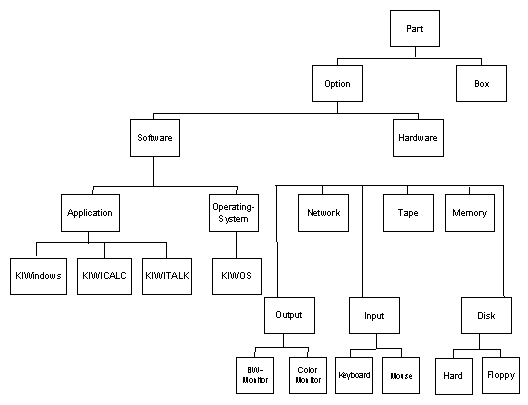
\includegraphics[scale=0.7]{f2-1}
  \caption{Example of a Single Inheritance Hierarchy}
  \label{f:2-1}
\end{figure}

Table~\ref{t:inchar} lists all the characteristics of object classes and
attributes that can be inherited by a subclass. Default
values can be \emph{redefined} by a subclass; the declaration in the
subclass overrides the declaration in the parent class for
that subclass and for all classes inheriting from it.
Attribute structure cannot be redefined; it is a compile-time
error to try to redefine a scalar attribute to be compound,
or vice-versa.
\begin{table}[h]
  \begin{tabularx}{\columnwidth}{Xcl}
    \toprule
    Characteristic              & Can be Redefined?      & Details in section\ldots   \\
    \midrule
    Membership in the parent class    & No          & Object Class Hierarchy \\
    Attribute names             & No          & Attributes   \\
    Attribute structure         & No          & Compound Attributes     \\
    Data type of each attribute & No          & Data Type Declaration    \\
    Default value of each attribute       & Yes         & Default Value \\
    \bottomrule
  \end{tabularx}
  \caption{Inherited Characteristics}
  \label{t:inchar}
\end{table}  

RuleWorks provides an implicit top-level object class called
\verb|$ROOT|. Any object class that you declare without an explicit
\tt{INHERITS-FROM} clause is treated as though you declared the parent
class \verb|$ROOT|. Figure~\ref{f:2-2} shows the implied hierarchy for
the top-level user-declared object classes in the sample program
\tt{KIWI.RUL}.

The specificity of a class is measured by its distance from
\verb|$ROOT| in the inheritance hierarchy. Any top-level user-declared
object class, such as those shown in Figure~\ref{f:2-2} has class specificity
of one. Object classes \tt{SOFTWARE-OPTION} and \tt{HARDWARE-OPTION},
shown in Figure~\ref{f:2-1} have class specificity of three. Object
classes \tt{HD-30} and \tt{HD-200} have class specificity of six.

\begin{figure}[h]
  \centering
  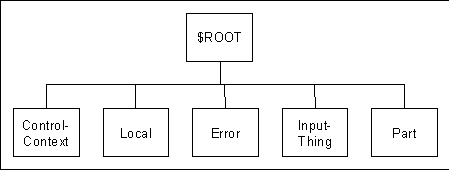
\includegraphics[scale=0.7]{f2-2}
  \caption{Inheritance from \tt{\$ROOT}}
  \label{f:2-2}
\end{figure}

\section{Working Memory Objects}

A working-memory object (WMO), sometimes called simply an
object, is a collection of attributes each with some value
(one or more atoms, or units of data) that represents a thing
or concept and its associated characteristics. In addition to
attributes with values, each object has a class name, an
identifier, and a time-tag. Figure~\ref{f:2-3} illustrates how
objects are stored in working memory.

\begin{figure}[h]
  \centering
  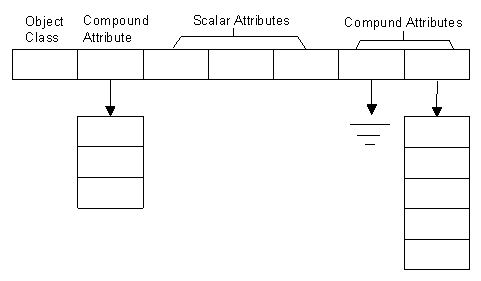
\includegraphics[scale=0.7]{f2-3}
  \caption{Conceptual Model of a Working-Memory Object}
  \label{f:2-3}
\end{figure}

\begin{quote}
  \textbf{Note:} The left-to-right order of the attributes shown in
  the figures do not necessarily reflect the actual internal
  representation. In RuleWorks you cannot depend upon the position of
  attributes in a WMO.
\end{quote}

All WMOs inherit two read-only attributes from the built-in
top-level class \verb|$ROOT|: \verb|^$ID| and \verb|^$INSTANCE-OF|. These
attributes store the instance identifier and class name of
the WMO (see Object Identifiers and Class Name)

RuleWorks displays WMOs in the following format:
\begin{quote}
\#\it{id} \it{time-tag} (\it{class-name} [\it{rule-name}] [\{\ct\it{attribute-name} \it{attribute-value}\} \ldots])
\end{quote}
For example:
\begin{qv}
#297 2529 (PERSON [INIT-DB] ^GIVEN-NAME LARRY ^LAST-NAME KIRK
  ^CHILDREN (COMPOUND ALEXANDER ALICIA ANDREW) ^SPOUSE NINA)
\end{qv}

RuleWorks does not include the names \verb|^$ID| and \verb|^$INSTANCE-OF|
when it displays a WMO, but it does include the values of
these attributes. RuleWorks does not display scalar
attributes whose value is \tt{NIL}, nor compound attributes that
have no elements, unless you have declared a default value
for the attribute (see Default Value Declarations for more on
default values).

\subsubsection*{Object Identifiers}

RuleWorks associates a unique identifier with each object
when it is created. This object identifier has the data type
\tt{INSTANCE-ID}. Unlike the time-tag, which is updated each time
the object is modified, the object identifier is guaranteed
to remain unchanged during the life of the object. Object
identifiers are stored in a built-in, read-only attribute
called \verb|^$ID|. It is an error to attempt to modify \verb|^$ID|.

A variable bound to an \tt{INSTANCE-ID} value is called an \tt{ID}
variable.

\tt{ID} variables can be compared for identity or non-identity,
as in the following rule, but nothing else:

\begin{example}[h]
\begin{qv}
(rule
  verify-configuration:kiwindows-needs-2-memory-cards-found-one
  ;This rule matches when there is exactly one object of class
  memory
  (active-context ^name verify-configuration)
  (kiwindows)
  (memory ^$id <mem-id>) ; there is one MEMORY
  -(memory ^$id <> <mem-id>) ; but there isn't another one
-->
  (make error ^severity warning ^message |Insufficient memory|)
  (write (crlf) |Caution: KiWindows requires two memory cards,|
         (crlf) | but you have only one memory card.|
         (crlf) | Fixup: adding another memory card to your order.|
         (crlf))
         (make memory))
\end{qv}
\caption{Comparing Object Identifiers}
\end{example}

\subsubsection*{Class Name}

A \emph{class name} is a symbol that identifies the class of which the
object is an instance. Objects that are instances of the same class
always have the same attributes, but the values of the attributes can
be different. The \tt{INSTANCE-ID} and time-tag of each object are
unique to that object.

Figure~\ref{f:2-4} shows seven different objects with the class name
\tt{CONTEXT}. Each of the seven has the same attribute, \verb|^NAME|,
but each has a different value for that attribute.

\begin{figure}[h]
  \centering
  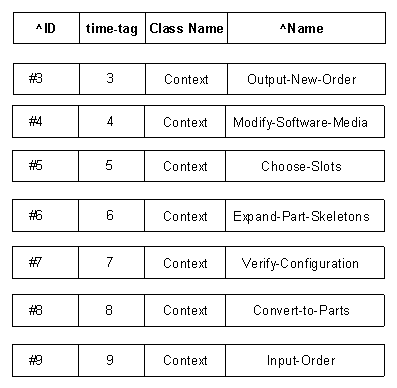
\includegraphics[scale=0.7]{f2-4}
  \caption{Multiple Objects of One Class}
  \label{f:2-4}
\end{figure}

The class name of an object is stored in a built-in,
read-only attribute named \verb|^$INSTANCE-OF|. You can use this
attribute on the LHS of a rule, but you cannot modify it.

\subsubsection*{Time-Tags}

\emph{Time-tags} are integers that the run-time system uses to
determine recency during conflict resolution. You cannot match or
modify time-tags. The run-time system assigns a unique time-tag to
each object in working memory. The time-tag is automatically updated
whenever the object is modified. Therefore, the object with the
largest time-tag is the most recently created or changed.

\section{Attributes}

An attribute consists of the attribute operator (\verb|^|) followed
by an attribute name that describes a characteristic of the
object class. Attribute names are symbols and are declared in
the \tt{OBJECT-CLASS} declaration.

Attributes can be declared in a parent class or in any
inheriting subclass. For example, all components of the
Kiwi-9200 share some attributes by virtue of being a \tt{PART}.
These attributes (\verb|^PART-NUMBER|, \verb|^NAME|, \verb|^PRICE|, and
\verb|^IS-EXPANDED|) are specified in the \tt{OBJECT-CLASS} declaration
of \tt{PART} and propagated down from \tt{PART} to \tt{OPTION}, to
\tt{HARDWARE-OPTION} and \tt{SOFTWARE-OPTION}, and so on, by
inheritance. The attributes that distinguish hardware from
software are specified in separate \tt{OBJECT-CLASS} declarations.
(See Example~\ref{e:declattr})

\begin{example}[h]
\begin{quote}
\begin{verbatim}
;The OBJECT-CLASS HARDWARE-OPTION. Hardware-options
;have to know whether they take up a slot in the
;CPU box, whether they have been placed in a slot,
;and what slot they are in.

(object-class hardware-option
    (inherits-from option)
    ^takes-slot
    ^is-placed
    ^in-slot)

;The OBJECT-CLASS SOFTWARE-OPTION. All software
;options have a media type as well as the
;other attributes inherited from OPTION and PART.

(object-class software-option
    (inherits-from option)
    ^media-type)
\end{verbatim}
\end{quote}
\caption{Declaring Additional Attributes}
\label{e:declattr}
\end{example}

Suppose you want to specify an object that has the class name
KIWICALC, is distributed on a 3.5-inch floppy disk, has part
number S-CA-9200, name KiwiCalc Spreadsheet Software, price
{\$}29.95, and a status flag whose value is \tt{YES}. You can specify
this object as shown in the example.

\begin{example}[h]
\begin{quote}
\begin{verbatim}
(kiwicalc ^media-type FD-35
          ^part-number S-CA-9200
          ^name |KiwiCalc Spreadsheet Software|
          ^price 29.95
          ^is-expanded yes)
\end{verbatim}
You can declare this object class as follows:
\begin{verbatim}
(object-class kiwicalc
    (inherits-from kiwos-application))
\end{verbatim}           
In this example, all the attributes are inherited. For a detailed
description of the \tt{OBJECT-CLASS} declaration, see
Chapter~\ref{c:conditionelements} of this manual.
\end{quote}
\caption{Specifying an Object}
\label{e:specobj}
\end{example}

Attributes are local to an object class and its descendants;
you can use the same attribute name in unrelated object
classes. For example, the attribute \verb|^NAME| is used in both of
the following objects:
\begin{qv}
(context ^name input-order)
(kiwicalc ^media-type fd-35 ^name kiwicalc)
\end{qv}

\subsubsection*{Scalar Attributes}

The value of a scalar attribute is a single atom (see the
section Atoms). For example:
\begin{qv}
^name |KiwiCalc Spreadsheet Software|
^price 29.95
\end{qv}
The values of these attributes are the symbolic atom
\verb,|KiwiCalc Spreadsheet Software|, and the floating-point atom
29.95. The figure shows how the run-time system stores the
scalar attribute values for a \tt{KIWICALC} object.

\begin{figure}[h]
  \centering
  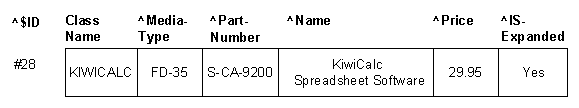
\includegraphics[scale=0.7]{f2-5}
  \caption{Storing the Values of Scalar Attributes}
  \label{f:2-5}
\end{figure}

\subsubsection*{Compound Attributes}

A \emph{compound attribute} contains a dynamically-sized, ordered
collection of scalar values. Such a collection is called a
\emph{compound value}. When a compound attribute is bound to a
variable, the variable is called a \emph{compound variable} and has a
compound value. The individual scalar atoms are called \emph{elements}
of the compound value.

Compound values are created (and displayed) with the \tt{COMPOUND}
function. For example:
\begin{qv}
  (compound memory memory keyboard fd-35)
\end{qv}

RuleWorks does not have multilevel lists like LISP; the
result of concatenating the compound value \tt{(COMPOUND A B C)},
the atom \tt{D}, and the compound value \tt{(COMPOUND E F)} is the
compound value \tt{(COMPOUND A B C D E F)}, not the multilevel
list \tt{((A B C) D (E F))}.

Figure~\ref{f:2-6} shows a conceptual model of an object class that
has two compound attributes.

\begin{figure}[h]
  \centering
  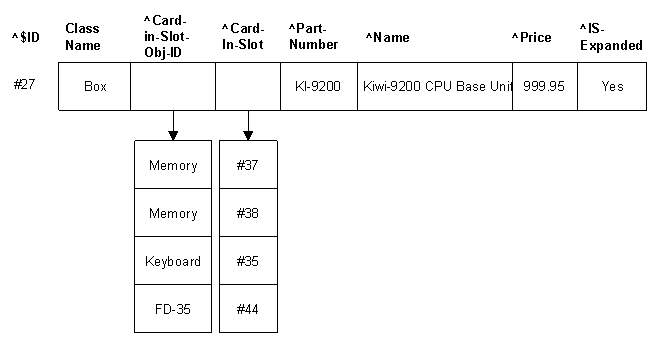
\includegraphics[scale=0.7]{f2-6}
  \caption{Conceptual Model of Compound Attributes}
  \label{f:2-6}
\end{figure}

The object in Figure~\ref{f:2-6} has the class name \tt{BOX}; the scalar
attributes \verb|^PART-NUMBER|, \verb|^NAME|, \verb|^PRICE|, and
\verb|^IS-EXPANDED|; and the compound attributes \verb|^CARD-IN-SLOT|
and \verb|^CARD-IN-SLOT-OBJ-ID|. Note that the left-to-right order of
the attributes in the figure does not necessarily reflect the actual
internal representation of an object. The top-down order of the values
in the compound attributes, however, does match the actual
representation. Compound attributes are indexed starting at 1 (not
0). The first element of \verb|^CARD-IN-SLOT| has the value
\verb|MEMORY|; the fourth and last has the value \verb|FD-35|.

There is no preset limit on the number of atoms allowed in compound
attributes; their size is limited only by memory available. You do not
need to allocate memory for them. The size of a compound value varies
during a program's execution.  See Chapter~\ref{c:conditionelements}
for information on matching compound attributes; see Chapter 4 for
information on creating and changing compound values.

Use the \tt{COMPOUND} keyword in an \tt{OBJECT-CLASS} declaration to
define the name of a compound attribute.

\begin{example}[h]
\begin{qv}
(object-class box
    (inherits-from part)
    ^card-in-slot compound
    ^card-in-slot-obj-id compound)
\end{qv}
\caption{\tt{OBJECT-CLASS}}
\end{example}

The compound attribute declaration is local to the object
class (and its inheriting subclasses), so it is possible for
an attribute name to be compound in one object class and
scalar in another. It is not possible for an attribute to be
compound in the parent class but scalar in a subclass, or
vice-versa.

\subsubsection*{Data Type Declarations}

By default, the value of a scalar attribute can have any
valid atomic data type, and the value of a compound attribute
can be a mixture of data types. RuleWorks uses a weak typing
system for attribute values. That is, data type declarations
are not required but if you provide one, RuleWorks enforces
it.

Data types can be added to the \tt{OBJECT-CLASS} declaration after
the attribute name whose type you want to specify as shown in
the following:.

\begin{quote}
  \verb|(object-class| \it{class-name} \{\verb|^|\it{attribute-name}
    [\verb|COMPOUND|] \it{data-type}\} \ldots \verb|)|
\end{quote}

For example:

\begin{quote}
\begin{verbatim}
(object-class person
    ^name symbol
    ^age integer
    ^children compound symbol)
\end{verbatim}
\end{quote}

Table~\ref{t:2-2} shows the symbols that can be used in data type
declarations for attributes.

\begin{table}[h]
  \centering
  \begin{tabular}{lll}
    \toprule
    Data Type & Description & Default value \\
    \midrule
    \tt{INTEGER}     & Integer number        & 0             \\
    \tt{FLOAT}       & Floating point number & 0.0           \\
    \tt{NUMBER}      & Either kind of number & 0             \\
    \tt{SYMBOL}      & Symbolic atom         & \tt{NIL}           \\
    \tt{INSTANCE-ID} & Object identifier     & \verb|#0|     \\
    \tt{OPAQUE}      & Virtual address       & \verb|%x0|    \\
    \tt{ANY}         & Any of the above      & \tt{NIL}           \\  
    \bottomrule
  \end{tabular}
  \caption{Data Types for Attributes}
  \label{t:2-2}
\end{table}

RuleWorks does not perform automatic coercion on values
assigned to typed attributes, not even between integers and
floats. To ensure that a value has the correct type, use one
of the built-in coercion functions: \tt{FLOAT}, \tt{INTEGER}, or
\tt{SYMBOL}.

\subsubsection*{Default Value Declarations}

When you create an object, you do not need to specify a value
for each attribute. RuleWorks supplies a default value for
attributes whose values were not specified. You can specify
the default value for each attribute, or use RuleWorks's
default.

If an attribute does not have a data-type declaration, the default
value is the \tt{NIL} for scalar attributes and the empty list
(\tt{(COMPOUND)}) for compound attributes. If an attribute has a data
type declaration but does not have default value declaration, its
default value depends on its data type (see Table~\ref{t:2-2}).

You specify a default value for an attribute with the \tt{DEFAULT}
keyword in the \tt{OBJECT-CLASS} declaration. The following
example shows the declaration of the \tt{PART} class from the
sample configuration program.

\begin{example}[h]
\begin{qv}
(object-class part
    ^part-number
    ^name
    ^price 
    ^is-expanded (default no))
\end{qv}
\caption{Declaration of the \tt{PART} Class}
\end{example}

When any object that inherits from class \tt{PART} is made, and no
new value for the \verb|^IS-EXPANDED| attribute is specified, the
value of that attribute is \tt{NO}.

For a compound attribute, the specified default value is
itself a compound value that will be used as the initial
contents of the attribute, if none is specified in the \tt{MAKE}
action. The following example declares an initial value for
the hypothetical compound attribute \verb|^TASKS|:

\begin{example}
\begin{qv}
(object-class agenda
    ^tasks compound symbol
       (default (compound input-order
                          convert-to-parts
                          verify-configuration
                          expand-part-skeletons
                          choose-slots
                          modify-software-media
                          output-new-order)))
\end{qv}
\caption{Declaring an Initial Value for \ct\tt{TASK}}
\end{example}

\subsubsection*{Fill Value Declarations}

You can modify a compound attribute by specifying a new value for any
element. Thus, it is possible to modify a compound attribute``beyond''
the last assigned element. The question arises, what value do elements
between the former end and the new end of the compound now have? To
answer this question, RuleWorks allows you to declare a \emph{fill},
or placeholder, value for the compound attribute.

RuleWorks' default fill value depends on the data type of the compound
attribute, if any. You specify a different fill value in the
\tt{OBJECT-CLASS} declaration, after the \tt{COMPOUND} keyword. For
example, consider the declaration shown below:
\begin{qv}
(object-class agenda
    ^tasks compound
       (default (compound input verify output))
       (fill no-op))
\end{qv}
When an \tt{AGENDA} object is made, the default value of its
\verb|^TASKS| attribute is \tt{(COMPOUND INPUT VERIFY
  OUTPUT)}. Suppose the following \tt{MODIFY} action is executed:
\begin{qv}
(modify <my-agenda> ^tasks[5] clean-up)
\end{qv}
The value of \verb|^TASKS| is now \tt{(COMPOUND INPUT VERIFY OUTPUT
  NO-OP CLEAN-UP)}.

Default Value Declarations explains how to specify a default value for
the entire compound attribute.

\section{Value Expressions}

In RuleWorks an attribute value can be set by using a constant, a
variable, an arithmetic expression, a function call, or an expression
that contains any of these things.

\subsection{Atoms}

The smallest unit of data in a RuleWorks program is called an
atom. Atoms must be one of the data types listed in Table~\ref{t:2-2}.

\subsubsection{Symbolic and Quoted Atoms}

A symbolic atom is one that does not have a numeric value. A symbol
consists of from 0 to 256 printable ASCII characters on a single
line. For example:
\begin{qv}
c
PLANT
?-c
10-14
\end{qv}
RuleWorks supports the eight-bit DEC Multinational Character
Set. Table~\ref{t:2-3} lists the characters that cannot be used in
unquoted RuleWorks symbols.

\begin{table}[h]
  \centering
  \begin{tabular}{ll}
    \toprule
    Character & Description \\
    \midrule
    Parenthesis (\verb|()|) & Enclose rules, actions, and so on. \\
    Braces (\verb|{}|) & Indicate conjunctions. \\
    Brackets (\verb|[]|) & Index compound attributes. \\
    Caret (\verb|^|) & The attribute operator. \\
    Semicolon (\verb|;|) & The comment character. \\
    Vertical bar (\verb,|,) & The quote character. \\
    Pound sign (\verb|#|)  & Indicates an instance identifier. \\
    Percent sign (\verb|%|) & Indicates an opaque address. \\
    White space & Tokens (space, tab, line feed, form feed, vertical tab). \\
    Ampersand (\verb|&|) & Reserved for future use.  \\
    Double-quote (\verb|"|) & Reserved for future use. \\
    Tilde (\verb|~|) & Reserved for future use. \\
    \bottomrule
  \end{tabular}
  \caption{Special Characters}
  \label{t:2-3}
\end{table}

\begin{quote}
  \textbf{Note:} RuleWorks does not support null characters in any
  symbol, quoted or not.
\end{quote}

To include special characters or white space in an atom, quote the
atom by enclosing it in vertical bars (\verb,||,). The text between
the two vertical bars is considered to be one symbolic atom. For
example, the compiler and run-time system recognize
\verb|THIS IS AN ATOM;| \verb|THIS IS NOT| to be four symbolic atoms followed
by a comment, which they ignore. However, they recognize
\verb,|THIS IS AN ATOM;, \verb,THIS IS NOT|, to be a single symbolic
atom.

Quoted atoms are symbolic atoms; therefore, \verb,|1.2|, is a symbol,
not a floating-point number, and arithmetic operations cannot be
performed on it. The opening and closing vertical bars, which can
enclose as many as 256 characters, must appear on the same line in the
code. The empty symbol are vertical bars enclosing nothing
(\verb,||,).

To quote a vertical bar itself, double it. For example:
\begin{qv}
|This is a vertical bar - ||.|
\end{qv}
When this atom is displayed or printed, it includes only one
vertical bar:
\begin{qv}
This is a vertical bar - |.
\end{qv}
When reading unquoted symbols, RuleWorks automatically turns lowercase
characters into uppercase. An unquoted symbol printed by RuleWorks may
appear to be different from the symbol read by RuleWorks. If you want
the print form to be the same as the read form, you must use quoted
symbols. Table~\ref{t:2-4} shows the read and print forms of several atoms.

\begin{table}[h]
  \centering
  \begin{tabular}{lll}
    \toprule
    Read Form & Print Form & Data Type \\
    \midrule
    \verb,A, &  \verb,A, & \tt{SYMBOL} \\
    \verb,a,        & \verb,A,          & \tt{SYMBOL} \\
    \verb,|a|,       & \verb,a,          & \tt{SYMBOL} \\
    \verb,|a b|,     & \verb,a b,        & one \tt{SYMBOL} \\
    \verb,a b,       & \verb,A B,        & two \tt{SYMBOL}s \\
    \verb,|A B|,     & \verb,A B,        & one \tt{SYMBOL} \\
  \bottomrule
  \end{tabular}
  \caption{Read Forms and Print Forms}
  \label{t:2-4}
\end{table}

All atoms that are not symbols have read forms that are identical to
their print forms.

\subsubsection{Integer Atoms}

Integer atoms consist of the following:
\begin{itemize}
\item An optional plus or minus sign
\item One or more decimal digits
\item An optional decimal point
\end{itemize}

The following are examples of integer atoms:
\begin{qv}
0
25.
-14
-5.
\end{qv}
Integer atoms can represent the same range of values as a ``long'' in
the C language. On Digital UNIX for Alpha, integers are 64 bits. That
is, the valid range for integer atoms is $-2^{63}$ to $2^{63}- 1$. On
all other systems, integers are 32 bits or $-2^{31}$ to $2^{31}-1$.

\subsubsection{Floating-Point Atoms}

A floating-point atom is composed of the following:
\begin{itemize}
\item An optional plus or minus sign
\item Zero or more decimal digits
\item A decimal point
\item Either one or both of these:
  \begin{itemize}
  \item One or more decimal digits after the decimal point
  \item An optional exponent
  \end{itemize}
\end{itemize}
An exponent consists of the letter ``E'' followed by a signed
or unsigned integer and represents a power of 10 by which a
preceding number is to be multiplied. For example, E-8
represents the value 10 raised to the power -8.

\begin{quote}
  \textbf{Note:} A floating-point atom must include a decimal point
  followed by a digit or an exponent, or both.
\end{quote}

The following are examples of floating-point atoms:
\begin{qv}
0.0
.25
10.05e-14
-5.e10
\end{qv}
Floating-point numbers are stored in double-precision and can
represent the same range of values as a ``double'' in the C
language. (On VAX systems, this is \verb|D_float data|; see the
\emph{VAX Architecture Handbook}. On Alpha systems, this is
\verb|G_float| data; see the \emph{Alpha Architecture Handbook}.)

\subsubsection{Instance Identifier Atoms}

Values of type \tt{INSTANCE-ID} are used to identify objects.
RuleWorks displays (and you type) an \tt{INSTANCE-ID} atom as a number
sign (\verb|#|) followed by an integer.
\begin{qv}
#1
#7955
\end{qv}

\begin{quote}
  \textbf{Note:} \tt{INSTANCE-ID}s are not integers. Arithmetic
  operations cannot be applied to values of type \tt{INSTANCE-ID}, and
  they cannot be compared except for identity or nonidentity.
\end{quote}

More information on variables bound to atoms of type \tt{INSTANCE-ID}
is found in Chapter~\ref{c:conditionelements}.

\subsubsection{Virtual Address Atoms}

Values of type \tt{OPAQUE} store addresses of functions or
external data structures. An \tt{OPAQUE} value is an ``atomic
address'' or in C terms, a ``void *''.

The print form of an \tt{OPAQUE} atom is a percent sign and an \verb|x|
(\verb|%x|) followed by a string of hexadecimal digits. The size of
\tt{OPAQUE} atoms depends on the machine architecture you are
using. Note that \tt{OPAQUE} may or may not be the same size as
the \tt{INTEGER} data type.

There is no way in RuleWorks directly to create a constant of
type \tt{OPAQUE}, except for the null pointer which is a RuleWorks
constant. For example:
\begin{qv}
%x0 ; the null pointer
\end{qv}
An \tt{OPAQUE} constant can be passed into RuleWorks from an
external routine, or as an input argument to an entry block,
and then passed out or returned.

\begin{note}
  \tt{OPAQUE} atoms are not numbers. Arithmetic operations cannot be
  applied to values of type \tt{OPAQUE}, and they cannot be compared
  except for identity or nonidentity.
\end{note}

\subsection{Variables}

A variable is any unquoted symbol enclosed in angle brackets
(\verb|< >|). An example is \verb|<PRICE>|.

\begin{note}
  In RuleWorks, the symbols \verb|<=>| and \verb|<->| represent the
  same-type and different-type operators. They cannot be used as
  variables.
\end{note}

You can use a variable as an argument to an action if the variable is
bound to a value. A variable can be bound to a value in a condition
element or in a \tt{BIND} action.

The following \tt{WRITE} action has two arguments: a quoted symbolic
atom and a bound variable.
\begin{qv}
(write |The value found was:| <x>)
\end{qv}

\subsection{Arithmetic Expressions}

Arithmetic expressions can be used anywhere a numeric constant may be
used. An arithmetic expression can contain numbers, variables bound to
numbers, functions which return numbers, and arithmetic operators. The
expression must be enclosed in parentheses, except when indexing into
a compound value. For example:
\begin{qv}
^price = (<item-1> + <item-2>) ; add two bound variables
^card-in-slot[<n> + 1] memory ; add a variable and a constant
\end{qv}
The valid operators are:
\begin{table}[h]
  \centering
  \begin{tabular}{ll}
    \toprule
 Operator & Description    \\
    \midrule
    \verb|+|        & Addition       \\
    \verb|-|        & Subtraction    \\
    \verb|*|        & Multiplication \\
    \verb|/|        & Division       \\
    \verb|\|        & Modulus        \\
    \bottomrule
  \end{tabular}
  \caption{RuleWorks Operators}
\end{table}

If an expression contains both integers and floating-point numbers,
the result is a floating-point number. If an expression contains
integers only, the result is an integer (by truncation). For example,
7.0 (float) divided by 4 (integer) is 1.75 (float), but 7 (integer)
divided by 4 (integer) is 1 (integer).
\begin{note}
Use the modulus operator only with integer operands.
\end{note}
Use infix notation in RuleWorks arithmetic expressions, that is, place
operators between operands. Separate each operator and operand with a
space. Surround the entire expression with parentheses. For example:
\begin{qv}
(2 + <X>)
\end{qv}
Spaces are not required around any of the special characters in the
first five rows of the table.

Expressions are evaluated from left to right. Precedence of operators
follows the normal conventions:

\begin{quote}
\verb|-|  ; unary negation, highest precedence

\verb|*| \verb|/| \verb|\| ; multiplication, division, and modulus

\verb|+| \verb|-|  ; addition and subtraction, lowest precedence
\end{quote}

For example, the following expression evaluates to 12, not 20:
\begin{qv}
(2 + 2 * 5)
\end{qv}
To override the normal precedence, use more parentheses. The following
expression does evaluate to 20:
\begin{qv}
((2 + 2)* 5)
\end{qv}
Consider the following rule:
\begin{quote}
\begin{verbatim}
(rule choose-slots:place-memory
    (active-context ^name choose-slots)
    (box ^$ID <the-box> ^card-in-slot { [=] <len> [<] 6 })
    (memory ^$ID <the-mem> ^is-placed nil ^takes-slot yes)
  -->
    (modify <the-box>
        ^card-in-slot [ ( <len> + 1 ) ] memory
        ^card-in-slot-obj-id [ ( <len> + 1 ) ] <the-mem>)
    (modify <the-mem> ^is-placed yes ^in-slot ( <len> + 1 )))
\end{verbatim}
\end{quote}
    
The \tt{MODIFY} actions in this rule use numeric expressions for
the index into a compound attribute and for the value of a
scalar attribute.

\begin{note}
  RuleWorks does not have complex mathematical functions built in. For
  example, RuleWorks has no \tt{ARC-COSINE} function.  For such
  complex mathematical functions, a RuleWorks program can call
  external routines written in other languages that are optimized for
  algorithmic coding.
\end{note}

\subsection{Function Calls}

The format for specifying a function call is:
\begin{quote}
\verb|(|\it{function-name} \it{argument-1} \it{argument-2} \ldots\verb|)|
\end{quote}
Use the same format whether the function is built-in or user-defined
(as an external function or an entry block that returns a value).
\begin{note}
  If a function requires no arguments, you must still enclose the
  function name in parentheses.
\end{note}
You can represent a value with a call to a built-in RuleWorks
function. Consider the following \tt{MAKE} action:
\begin{qv}
(make input-thing ^item (accept-atom infil))
\end{qv}
First, the run-time system evaluates the call to the \tt{ACCEPT-ATOM}
function. The \tt{MAKE} action then stores the value returned by the
\tt{ACCEPT-ATOM} function in the \verb|^ITEM| attribute of the
\tt{INPUT-THING} object it creates.

You can also represent a value with a call to a user-defined function,
written in RuleWorks or some other language. In either case, you must
declare the function before you call it. The following \tt{BIND}
action calls the external function \verb|SQUARE-ROOT|:
\begin{qv}
(bind <std-deviation> (square-root <variance>))
\end{qv}

%%% Local Variables:
%%% mode: latex
%%% TeX-master: "rwug"
%%% End:
